%--------------------------------------------------------------------------------------------
%   YART thesis LaTeX document main entry point.
%
%   Contains global configuration, imports and document structure definition. 
%--------------------------------------------------------------------------------------------

\documentclass[twoside, 12pt]{report}

% +===+ GLOBAL PACKAGE IMPORTS +===+ % 
\usepackage[utf8]{inputenc}

\usepackage[top=2cm, bottom=3cm]{geometry} % For defining custom document geometry
\usepackage[backend=biber,style=numeric-comp,sorting=none]{biblatex} % For citations using BibTeX
\usepackage{tikz} % For defining and drawing diagrams
\usepackage{bm} % For bold symbols in maths mode
\usepackage{listings} % For defining custom listing styles 
\usepackage{graphicx} % For including graphics
\usepackage{subcaption} % For displaying figures side by side
\usepackage{hyperref} % For hyperlink generation
\usepackage[noabbrev, capitalise]{cleveref} % For \cref
\usepackage{setspace} % For paragraph indentation
\usepackage{fancyhdr} % For a custom header/footer formatting
\usepackage{titlesec} % For defining custom section formats
\usepackage{tocloft} % For table of contents and table of figures style formatting
\usepackage[indent=24pt]{parskip} % For paragraph indentation


% +===+ SETUP BibTeX FOR CITING +===+ %
\addbibresource{references.bib}
\emergencystretch=1em % https://tex.stackexchange.com/questions/171999/overfull-hbox-in-biblatex


% +===+ SETUP TikZ FOR DIAGRAM DRAWING +===+ %
\usetikzlibrary{positioning, fit, arrows.meta, backgrounds}

% Declare default render layers
\pgfdeclarelayer{background} 
\pgfdeclarelayer{foreground}
\pgfsetlayers{background, main,foreground}

% Declare global style
\tikzstyle{module}=[draw, thick, fill=blue!5, rounded corners, inner sep=8pt, font=\bfseries\small]
\tikzstyle{main}=[draw, rounded corners, font=\large, minimum width=10cm, minimum height=1cm]
\tikzstyle{component}=[main, fill=yellow!10, dashed]


% +===+ CUSTOM LISTINGS FORMATTING +===+ %
\lstset{%
    language=C++,
    basicstyle=\small,
    numberstyle=\footnotesize,
    commentstyle=\color{darkgray},
    columns=fullflexible,
    aboveskip=1.5\bigskipamount,
    belowskip=\smallskipamount,
    lineskip=0.5mm,
    numbers=left,
    numbersep=1em,
    showspaces=false,
    showstringspaces=false,
    showtabs=false,
    frame=lines,
    tabsize=4,
    captionpos=b,
    breaklines=true,
    breakatwhitespace=false,
    escapeinside={\%*}{*)}
}

% Change the list of listings title name
\renewcommand{\lstlistlistingname}{List of Listings}


% +===+ CUSTOM STYLE FORMATTING +===+ %
\raggedbottom % Automatically add vertical spacing at the end of every page 

% Custom chapter format
\titleformat{\chapter}[display]
    {\normalfont\bfseries\Large\centering}
    {\sc Chapter \thechapter}{-10pt}
    {\MakeUppercase}

% Custom page numbering format
\pagestyle{fancyplain}
\fancyhf{} % Clear the default fancy style 
\renewcommand{\headrulewidth}{0pt} % Remove the header rule
\fancyfoot[RE, LO]{\thepage}

% Custom table of contents format
\renewcommand{\cftchapleader}{\cftdotfill{\cftdotsep}} % Dotted lines for chapters in TOC
\renewcommand\cfttoctitlefont{\hfill\Large\bfseries\MakeUppercase}
\renewcommand\cftaftertoctitle{\hfill\mbox{}}
% \renewcommand{\contentsname}{Table of Contents}

% Custom table of figures format
\renewcommand\cftloftitlefont{\hfill\Large\bfseries\MakeUppercase}
\renewcommand\cftafterloftitle{\hfill\mbox{}}


% % +===+ CUSTOM COMMANDS AND COLOR DEFINITIONS +===+ %
\newcommand\blankpage{ % Inserts a blank page
    \null\thispagestyle{empty}
    \addtocounter{page}{-1}
    \newpage
}

% Colors for coordinate system diagrams
\definecolor{axis_red}{RGB}{244, 36, 84}
\definecolor{axis_green}{RGB}{84, 244, 36}
\definecolor{axis_blue}{RGB}{36, 84, 244}


% +===+ DOCUMENT STRUCTURE +===+ % 
\begin{document}
    %--------------------------------------------------------------------------------------------
%   YART thesis title page definition.
%--------------------------------------------------------------------------------------------

% === CUSTOM \maketitle DEFINITION === %
\renewcommand{\maketitle} {
    % +===+ TITLE PAGE CUSTOM GEOMETRY +===+ %
    \newgeometry{margin=2.5cm,top=3.5cm,bottom=3.0cm}

    \begin{titlepage}
        \begin{center}
            % +===+ UNIVERSITY & FACULTY NAME +===+ %
            \textsc{ 
                \Large UNIVERSITY OF SILESIA IN KATOWICE \\
                \large FACULTY OF SCIENCE AND TECHNOLOGY
            }
    
            \vspace{3.5cm}

            \textsc{\LARGE{Bachelor's Thesis}}
            
            \vspace*{0.5cm}
            
            % +===+ THESIS TITLE +===+ %
            \rule{\linewidth}{0.2mm}\\[0.2cm]
            \LARGE{\bfseries
                Implementation of a Ray Tracing Engine \\ 
                Using a CPU Based Renderer \\[0.2cm]
            }
            \rule{\linewidth}{0.2mm}

            \vspace*{1.0cm}

            % +===+ AUTHOR & SUPERVISOR +===+ %
            \begin{minipage}[t]{0.37\textwidth}\raggedright\large
                \textit{Author} \\
                Dawid \textsc{Cyganek} \\
                \normalsize{(338241)}  
            \end{minipage}
            \begin{minipage}[t]{0.37\textwidth}\raggedleft\large
                \textit{Supervisor} \\
                Dr. Krzysztof \textsc{Górny}
            \end{minipage}
            
            \vspace*{1.0 cm} 

            \vspace*{\fill} % float to bottom of the page
            
            \normalsize{
                January 1, 2024 \\
                Katowice
            }

        \end{center}
        
        \clearpage
    
    \end{titlepage}

    \restoregeometry
}


% +===+ RENDER THE TITLE PAGE +===+ %
\maketitle

    % \blankpage
    %--------------------------------------------------------------------------------------------
%   YART thesis abstract page definition.
%--------------------------------------------------------------------------------------------

\chapter*{abstract}
\addcontentsline{toc}{chapter}{ABSTRACT}

The purpose of this dissertation is to explore the world of ray tracing, focusing on fundamental principles of physically-based rendering and introducing a novel system called YART.
Designed to test the capabilities of modern CPUs, YART is an interactive 3D rendering application with an integrated ray tracing engine. 
The intricate creation process of such a system is described by delving into implementation detail of various key components of the YART engine, presented in a bottom-up approach.
Starting with the definition of a ray and ending in the implementation of a rendering loop, numerous algorithms are described along the way, such as ray-triangle intersection testing using M{\"o}ller-Trumbore, or the Blinn-Phong shading model. 

\vspace*{1em}

\noindent\textbf{Keywords:} Ray tracing, CPU, M{\"o}ller-Trumbore algorithm, Blinn-Phong algorithm

\clearpage

    \tableofcontents

    % \begin{onehalfspace}
        %--------------------------------------------------------------------------------------------
%   YART thesis "Introduction" chapter definition.
%--------------------------------------------------------------------------------------------

\chapter{Introduction} \label{ch:Introduction}

Vision is the single most advanced of human senses, which plays a vital role in determining how we perceive and experience the world.
It is not a surprise, that an ever-increasing amount of research and advancement has been made in pursuit of creating more photorealistic imagery in the field of computer graphics. 
In recent years, the dynamic landscape of computer graphics has witnessed a revolutionary shift with the rise and advancement of ray tracing technology. 
Unlike conventional rasterization techniques, ray tracing follows physical principles of light propagation, resulting in unparalleled level of visual realism. 

This dissertation aims to explore and elucidate the intricate inner workings behind a ray tracing engine, delving into the underlying principles and various considerations involved in the creation of such a system.
In contrast to a more conventional approach of implementing ray tracing within a specialized GPU pipeline, the proposed solution has instead been developed entirely on the CPU. 
Significant differences between these two types of implementations are noteworthy, especially in how they handle parallel processing, which can impact the performance and efficiency of a ray tracing application. 
While the highly parallel nature of a GPU is often preferred for commercial, real-time rendering systems, a CPU side implementation allows for gaining a deep understanding of fundamental principles of computer graphics, without the added complexity of GPU programming.

\section{Ray Tracing}

The concept of ray tracing has gained increased interest in most recent years, having seen a convergence of various advancements in hardware, algorithms, and an ever-growing industry demand for realism.
Its origin however, dates back to as far as 16th century, when it was first described by a german artist and theorist Albrecht Dürer \supercite{Hofmann1990}.
At its core, ray tracing is a graphics rendering technique, used to simulate the way light interacts with objects within a virtual environment. 
The process involves scattering rays of light from a virtual camera, tracing their paths as they travel and interact with a scene. 
Individual light rays are traced "backward", originating from the camera's viewpoint, as opposed to how they would be cast from a light source in a more realistic setting.
Doing so however, is many orders of magnitude more optimal, since only a small percent of rays emitted from a given light source actually make it directly into the camera's lens and contribute to the final image \supercite{Glassner1989}.
Each ray is then projected through a pixel on the output image plane, determining it's color by testing for intersections and sampling materials of hit objects.
This basic idea behind ray tracing is illustrated in \cref{fig:Introduction/RayTracing/rt1}. 

\vfill
\begin{figure}[!ht]
    \centering
    \includegraphics[width=0.8\textwidth]{example-image-a}
    \caption[Simplified ray tracing model]{Simplified ray tracing model.}
    \label{fig:Introduction/RayTracing/rt1}
\end{figure}
\vfill

When colliding with an object, the ray gets reflected of the surface, refracted, or absorbed depending on the hit object's material. 
Reflected rays are traced recursively to calculate the final color of a particular pixel, until being absorbed or reaching a certain limit of bounces.  

By following the physically-based principles of light, ray tracing enables straightforward simulation of highly realistic optical effects, such as refraction, depth of field and soft shadows.
This is in contrast to the traditional rendering method of rasterization, where producing similar results could be a difficult, or even an impossible task. 
The unmatched visual realism of ray tracing however does not come without cost. 
Ray tracing generally has a much greater computational cost, as compared to scanline rendering methods, which makes it a less performant algorithm of the two.
Until the late 2010s, creating an interactive ray tracing application for consumer hardware was generally considered as impossible.
Today, the ongoing development of commercial hardware and algorithmic advancements have made real-time ray tracing become feasible, making it a viable option for film production, video games, and commercial graphics applications.

\section{Related Work}

Numerous high-level ray tracing engines and APIs have been proposed for professional and commercial use since the dawn of physically-based computer graphics.
Each engine, having its distinct capabilities, purpose, and inherent limitations, has contributed greatly to the advancement of computer graphics. 
Following, is a list of noteworthy entries in the vast catalogue of existing ray tracing systems.

\subsection{NVIDIA OptiX}

First introduced in 2010, OptiX \supercite{Parker2010} is a programmable ray tracing framework developed for NVIDIA GPUs.
It has been designed with focus on both high flexibility and performance, targeting highly parallel hardware architectures.
The core idea behind the OptiX engine, is dividing the rendering pipeline into a small set of programmable operations or \textit{shaders}, akin to how rasterization pipelines are deployed within OpenGL and Direct3D applications.
These user-specified shaders can be defined to form a variety of ray tracing-based systems, including offline rendering, collision detection systems, and scientific simulations such as sound propagation.
For representing the scene, OptiX employs a lightweight data structure, called the \textit{context}, used for binding shaders to the object-specific data they require.
The context bundles together shaders, geometry data, and acceleration structures in the form of connected graph nodes, resulting in high flexibility and reusability.
While OptiX is a powerful tool for scientific research and professional ray tracing development, it may not be as user-friendly for artists and designers looking for out-of-the-box solutions.

\subsection{Intel Embree}

Embree \supercite{Wald2014}, is an open-source ray tracing framework developed at Intel, targeting x86 CPUs. 
Since its first release in 2011, it has become a cornerstone for a variety of leading 3D rendering applications. 
In contrast to NVIDIA's OptiX, which was designed to simplify development of new renderers, Embree aims to accelerate ray tracing in existing systems. 
This key design goal leads to highly optimized low-level kernels for accelerating ray generation and traversal that leverage modern CPU architectures.
All ray tracing operations supported by the Embree kernels can be accessed through an easy to use and compact API.
It exposes a number of functions for defining custom geometry and issuing intersection queries. 
The API aims to hide implementation detail such as data structure memory layout, while ensuring high performance intersection testing. 
Embree's lightweight and flexible API makes it in invaluable tool for developers seeking efficient ray tracing capabilities in their applications, without needing to worry about implementing lower-level optimizations and acceleration structures.

\subsection{Cycles}

Developed by the Blender Foundation, Cycles \supercite{Cycles} is an open-source ray tracing renderer, which can be integrated into commercial software. 
Since 2011, Cycles has been a part of the Blender 3D creation suite, and Blender's first physically-based rendering method.
It employs a \textit{path tracing} algorithm, which is a probability-based type of ray tracing.
Due to the unbiased nature and accuracy of the selected method, Cycles is able to naturally simulate highly realistic lighting scenarios, such as global illumination, soft shadows, and caustics.
Path tracing, is however prone to generating noise and requires a high number of samples to be made per pixel, until it can produce a relatively noise-free output.
In order to minimize the number of samples, while still ensuring accurate results, various denoising algorithms have been integrated into the engine, that aid in reducing noise artifacts in rendered images.
One of Cycles' standout features is its node-based material system, which provides users with a flexible and intuitive means of crafting advanced, physically accurate materials. 
Additionally, it supports GPU acceleration, which greatly improves the engine's performance, using the power of modern hardware.
The collaborative and open-source nature of Blender makes Cycles is a compelling choice for digital artists and designers seeking for a robust and accessible ray tracing solution.

\section{Outline}

This introductory chapter highlights the key purpose of this dissertation, provides background, and gives an outline of existing solutions. 
\cref{ch:Application} serves as a high-level overview of the proposed application, briefly describing its capabilities and architectural design. 
\cref{ch:Implementation} delves into implementation detail and various considerations involved with development of the ray tracing engine. 
The implementation has been divided into a set of smaller iterations, presented in an order a developer might follow when creating a new system.
Finally, \cref{ch:Conclusion} acts as the project's conclusion, describing possible future work, and giving a list of papers that might be found useful for further research.

        %--------------------------------------------------------------------------------------------
%   YART thesis "YART: A Ray Tracing Application" chapter definition.
%--------------------------------------------------------------------------------------------

\chapter{YART: A Ray Tracing Application} \label{ch:Application}

Proposed by this dissertation, \textit{Yet Another Ray Tracer} (YART) is a cross-platform 3D rendering application with an integrated ray tracing engine. 
It was build using the C++ programming language with a goal of exploring the inner workings of a ray tracing system and testing the capabilities of modern hardware.
The rendering engine has been entirely prepared on the CPU, using a traditional, object oriented approach.
As opposed to many state-of-the-art renderers which focus greatly on high performance and efficiency, YART is instead designed to be an easily customizable and scalable environment. 
While not prioritizing the engines performance, treading is used in various parts of the system to utilize the power of CPU parallelization.
In parts not directly related to ray tracing, the application's backend makes use of GPU capabilities for creating a window, and presenting subsequent frames onto it.
Additionally, YART aims to be highly interactive and verbose.
The application's graphical user interface (GUI) is designed to enable easy access to various parts of the engine, otherwise not exposed in similar, commercial software. 
YART's source code can be found in the project's \href{https://github.com/hhimko/yart}{official GitHub repository}. 

\section{Application Architecture}

YART's architecture can be divided into two key components.
The first of which, further referred to as the \textit{backend}, is dedicated to performing lower-level operations, such as opening and managing the application window, polling incoming inputs, as well as displaying application frames. 
It aims to abstract away platform-dependant functionalities, with the use of a lightweight API, designed to be implemented using various windowing systems and libraries. 
In general, the backend encapsulates every system-agnostic feature within YART, which could be related to GPU programming.

Everything beyond the backend, can be collectively referred to as the \textit{application core}. 
As the name implies, it consists of key application modules, which primarily include the ray tracing engine and the user interface.
The renderer does not directly depend on its system's backend, and vice versa. 
It has been designed to write its pixel output into an ordinary C-style array, not caring what happens to it afterwards.
Using this methodology, enables the renderer to be easily reused in various parts of the application, such as for rendering material preview viewports within the UI.

The backend and the application core are separated with the aim of decoupling system- and hardware-agnostic functionality from the rendering engine.
What binds them together, is a central \verb|yart::Application| class, designated to initializing both components and communicating between them using specialized callbacks. 
Furthermore, it introduces the \textit{mainloop}, which defines the fundamental control flow of every application frame.
The YART application architecture, with its components and relations made between them, is illustrated in \cref{fig:Application/ApplicationArchitecture/arch}. 

\begin{figure}[!ht]
    \centering
    \vspace*{3mm}

    \newcommand{\arrowshift}{95pt}

    \begin{tikzpicture}[auto]
        % Application core inner modules
        \node[module] (engine) {Ray Tracing Engine};
        \node[module, right=5mm of engine] (gui) {User Interface (UI)};

        \draw[->, thick] (gui) to (engine);

        % Application core label
        \node[draw=none, fit=(engine) (gui)] (core-modules) {};
        \node[font=\large, above=-1mm of core-modules, inner sep=4pt] (core-label) {Application Core};

        % Application core component
        \begin{pgfonlayer}{background}
            \node[component, fit=(core-modules) (core-label), minimum width=10cm] (core) {};
        \end{pgfonlayer}

        % Application class 
        \node[draw, rounded corners, inner sep=6pt, font=\bfseries\small, below=14mm of core, minimum width=97mm] (mainloop) {mainloop};
        \node[font=\large, above=0mm of mainloop, inner sep=4pt] (application-label) {\verb|yart::Application| Class};

        \begin{pgfonlayer}{background}
            \node[main, thick, fill=blue!5, fit=(mainloop) (application-label)] (application) {};
        \end{pgfonlayer}
        \draw[->, thick] ([xshift=\arrowshift]application.north west) to ([xshift=\arrowshift]core.south west);
        \draw[->, thick] ([xshift=-\arrowshift]core.south east) to ([xshift=-\arrowshift]application.north east);

        % Backend component
        \node[component, below=5mm of application] (backend) {Backend};
        \draw[<-, thick] ([xshift=\arrowshift]application.south west) to ([xshift=\arrowshift]backend.north west);
        \draw[<-, thick] ([xshift=-\arrowshift]backend.north east) to ([xshift=-\arrowshift]application.south east);
    \end{tikzpicture}

    \caption[YART application architecture]{YART application architecture.}
    \label{fig:Application/ApplicationArchitecture/arch}
\end{figure}

Introduction of the \verb|yart::Application| class implies, that the engine can be detached from the windowing backend, and easily transformed into other application types.
For example, the YART engine could be reused as an offline renderer within a new console application, or used as a ray tracing library in already existing systems.

\section{Functionality Overview}

YART allows for rendering complex, user-defined scenes, which mainly consist of mesh geometry, light sources and a customizable environment.
The application's UI introduces a set of tools and functionalities, which provide the end user with the ability to manage a scene, and customize various parts of the rendering engine.
Users can open new and empty scenes, and populate them with numerous primitives, such as cubes, spheres or planes.
Alternatively, a number of example scenes can be loaded via the application's main menu bar, and tailored depending on personal needs. 
The object hierarchy window displays all created scene objects and their individual properties, enabling further edition.
Objects selected in the hierarchy view can be freely translated and rescaled, allowing for a high variety of custom scenes.
Additionally, every object defines its own, customizable material, which influences its appearance and reflectance properties.
To avoid rendering scenes inside a black void, skies can be shaded using three methods employed in the engine: solid color skies, linear gradient skies, and textured skyboxes.
\cref{fig:Application/FunctionalityOverview/render_sample} illustrates a sample scene, rendered using the YART application's ray tracing engine.

\begin{figure}[!ht]
    \centering
    \includegraphics[height=9cm]{example-image-a}
    \caption[Example image rendered using the YART engine]{Example image rendered using the YART engine.}
    \label{fig:Application/FunctionalityOverview/render_sample}
\end{figure}

\section{External Dependencies}

All dependencies excluding Vulkan are included into, and built with the project, in the form of \textit{Git submodules}. 
Incorporated into the distributed version control system -- Git, submodules provide functionality to include separate Git repositories as subdirectories within another project.
The only closed-source dependency used within the project, is the Vulkan library.
In order for the application to build, the Vulkan software development kit (SDK) has to be installed on the users machine. 
Following, is a list of all external dependencies used throughout the YART application, including a brief description and their purpose within the project.

\subsection{GLFW}

GLFW \supercite{GLFW} is a lightweight C library for creating and managing windows.
It provides a multi-platform abstraction layer, primarily designed to work seamlessly with applications made using OpenGL \supercite{Neider1993}.
The GLFW API includes a straightforward mechanism for handing inputs such as keyboard or mouse, as well as various time management functions, making it easier to control the frame rate of an application.
YART makes use of GLFW to open a platform-specific window and handle all incoming user inputs. 
The window is used as a rendering surface, to which the GPU can draw subsequent application frames. 
GLFW exposes user input in the form of events, which can be polled and handled using specific callbacks. 
The event system is utilized within YART to handle key presses and mouse events for various interactions, such as viewing-camera movement and rotation.

\subsection{Vulkan}

Developed by the Khronos Group, Vulkan \supercite{Sellers2016} is a low-level graphics and compute programming interface.
Designed as a successor to the prominent OpenGL API, it provides an efficient and flexible framework for graphics programming on modern GPUs.
Unlike some higher-level graphics libraries, Vulkan does not hide, or abstract away the underlying hardware details or perform certain optimizations automatically. 
Instead, developers are equipped with high degree of control and responsibility.
Memory, synchronization, and devices have to be managed explicitly, leading to increased verbosity in the code.
Proper use of Vulkan capabilities can lead to better utilization of system resources and improved performance in graphics-intensive applications.

Vulkan, along with GLFW, serves as the window rendering backend for the YART application.
It does not however play any role in performing actual ray tracing computations, which are made entirely on the CPU. 
Instead, the backend utilizes the pixel output of the engine's renderer, which gets streamed into a texture and displayed every frame within a viewport.
For this purpose, a specialized graphics pipeline is deployed using Vulkan, that in its core, issues render commands to the GPU and presents frames to the GLFW window. The pipeline was designed to adapt to a high variety of hardware devices, taking advantage of their characteristics.
For example, depending on the capabilities of a physical device installed on the client's machine, multiple frames can be prepared in parallel, which can greatly improve the application's performance.
Querying these capabilities, allows the backend to optimize its render pipeline, and to target the most applicable device, in scenarios where multiple GPUs are available.

\subsection{Dear ImGui}

Dear ImGui \supercite{DearImGui}, is a versatile, open-source graphical user interface (GUI) library for the C++ language. 
It is fast, portable, and comes with a variety of UI components, that can easily be customized and styled.
ImGui is primarily designed as an interactive debugging tool for use in real-time rendering applications, video games, or other environments where GUI creation features are non-standard.
YART however, extends on Dear ImGui's standard feature set, to define custom widgets and render the final user interface layout. 
At its core, Dear ImGui is what makes the application interactive, enabling the end user to tinker with the engine's functionality.

\subsection{GLM}

OpenGL Mathematics (GLM \supercite{GLM}), is a C++ mathematics library designed specifically for graphics programming and game development.
It is lightweight, self contained, and header-only, meaning it does not use any external dependencies, and does not need to be separately compiled or linked.
YART benefits from vector and matrix operations available in GLM, which are essential for various rendering tasks, such as defining projections and calculating transformations.

        %--------------------------------------------------------------------------------------------
%   YART thesis "Implementation" chapter definition.
%--------------------------------------------------------------------------------------------

\chapter{Implementation} \label{ch:Implementation}

Before delving into the implementation of a ray tracing engine, certain considerations should be made, which will define the entire development workflow.
One such example is the choice of a coordinate system, that will affect the order of mathematical calculations.
Coordinate systems provide a standardized way of specifying locations and orientations of objects within a multi-dimensional environment.
In the context of two-dimensional computer graphics, the system typically consists of a X-axis pointing from left to right, and a Y-axis pointing upwards.
When adding the third coordinate however, the developer has a choice as to whether the Z-axis should point out of, or into the virtual screen, away from the viewer.
These two system types are respectively referred to as the right-handed coordinate system (RHS), and the left-handed coordinate system (LHS) (see \cref{fig:Implementation/coordinate_system}).
The names of these systems derive from the \textit{right-hand rule}, which is a convention used for determining the orientation of axes in three-dimensional space \supercite{RightHandRule}. 

\vfill
\begin{figure}[!ht]
    \centering

    \begin{subfigure}{.4\textwidth}
        \centering

        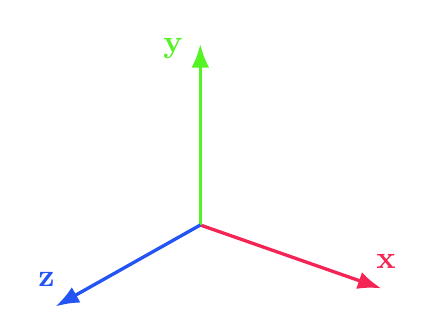
\begin{tikzpicture}[scale=1.15, every node/.style={scale=1.15}]
            \draw[-{Latex[length=3mm]}, color=axis_red, very thick]   (0, 0) -- (2, -0.7);
            \draw[-{Latex[length=3mm]}, color=axis_green, very thick] (0, 0) -- (0, 2);
            \draw[-{Latex[length=3mm]}, color=axis_blue, very thick]  (0, 0) -- (-1.6, -0.9);
            \node[color=axis_red] (x) at (2.05, -0.4) {\textbf{x}};
            \node[color=axis_green] (y) at (-0.3, 1.95) {\textbf{y}};
            \node[color=axis_blue] (y) at (-1.7, -0.6) {\textbf{z}};
        \end{tikzpicture}
        \caption{}
    \end{subfigure}%
    \begin{subfigure}{.4\textwidth}
        \centering
        
        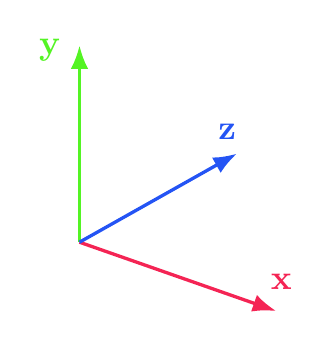
\begin{tikzpicture}[scale=1.25, every node/.style={scale=1.25}]
            \draw[-{Latex[length=3mm]}, color=axis_red, very thick]   (0, 0) -- (2, -0.7);
            \draw[-{Latex[length=3mm]}, color=axis_green, very thick] (0, 0) -- (0, 2);
            \draw[-{Latex[length=3mm]}, color=axis_blue, very thick]  (0, 0) -- (1.6, 0.9);
            \node[color=axis_red] (x) at (2.05, -0.4) {\textbf{x}};
            \node[color=axis_green] (y) at (-0.3, 1.95) {\textbf{y}};
            \node[color=axis_blue] (y) at (1.5, 1.12) {\textbf{z}};
        \end{tikzpicture}
        \caption{}
    \end{subfigure}

    \caption[RHS and LHS coordinate systems]{RHS (a) and LHS (b) coordinate systems.}
    \label{fig:Implementation/coordinate_system}
\end{figure}
\vfill

Both the RHS and LHS are commonly utilized in commercial rendering software.
While developing YART, the left-handed coordinate system has been used, solely based on personal preference. 
This information is important to keep in mind, as the choice of a system determines the definition and implementation of projections, and various matrix operations, used throughout a ray tracing engine. 

\section{Ray Definition}

The fundamental piece of any ray tracing engine is undeniably the concept of \textit{rays}.
In mathematics, a ray can be defined as a straight line extending infinitely in one direction from a specific starting point. 
It is therefore characterized by its origin point, and a unit vector denoting the directions it's facing.
Rays can be conceptualized across any number of dimensions, however for the specific application of ray tracing, we will only focus on three-dimensional rays.

Let's consider a ray with an origin point $ \bm{P} $, extending infinitely in the direction of a vector $ \bm{\hat{v}} $.
To sample a specific point along this ray, we define a function $ \bm{r} $
%
\begin{equation}
    \bm{r}(t) = \bm{P} + t\bm{\hat{v}}
\end{equation}
%
It returns all possible points on the ray, which are $ t $ units apart from its origin.
Knowing the distance from the ray's origin to the closest object hit along its path, function $ \bm{r} $ will enable us to find the exact point of collision on the object's surface.
For this purpose, it's important to make the direction vector $ \bm{\hat{v}} $ an unit vector, as a vector of length different than $ 1 $ would scale the distance proportionately, ultimately resulting in inaccurate calculations. 

In the code, we can define a ray as a lightweight structure containing two three-dimensional vector members, representing the ray's origin and direction (see \cref{lst:Implementation/RayDefinition/ray}).
This structure can later be extended with related operations, such as testing for ray-object intersections or reflecting of a given surface.

\vfill
\lstinputlisting[
    xleftmargin=1.5em, 
    caption={[Ray structure definition]
        Ray structure definition.},
    label={lst:Implementation/RayDefinition/ray}
]{include/listings/ListingRay.cpp}
\vfill

\section{Ray Generation and The Camera}

To render images using ray tracing methodology, generally means to trace a single ray for every pixel in the output image.
The color seen it the direction of those rays, is what defines the final color of their respective pixels. 
This initial phase of calculating ray directions for every image pixel, is often referred to as the \textit{ray generation} step of a ray tracing engine.
Ray generation in YART can be divided into four stages:
\begin{enumerate}
    \item defining and querying camera properties,
    \item computing a screen-space-to-camera-space transformation matrix,
    \item calculating individual ray directions using the matrix,
    \item caching the calculated direction vectors.
\end{enumerate}

\subsection{Camera Definition}

Before we can generate a ray, we first need to explain the basic concept behind a \textit{camera}.
Sometimes referred to as the \textit{eye}, a camera is the engine's virtual viewpoint, giving the ability to "see" into a digital environment.
At its core, it's used to generate rays for each pixel in the rendered image.
It is primarily represented by its position in world-space, a viewing direction (or \textit{look-at vector}), and the camera's field of view (FOV).
A camera's field of view represents the angular extent of the scene captured in the output image. 
FOV might be expressed in one of three different ways, as it can be measured horizontally, vertically, or diagonally.
The difference between them is significant, impacting the calculations made while defining a projection matrix.
In YART, horizontal measurement is used to determine camera's field of view.

The camera can be though of as a viewing context for rendering a scene.
Rays will be cast originating from the camera's position and traced in the direction it is facing, offset by \textit{screen-space} coordinates of subsequent image pixels.
Screen-space coordinates generally refer to a two-dimensional coordinate system that represents the positions of pixels on a screen.
In the context of ray tracing, the screen can be represented as an image, positioned at a specific distance from the camera's origin. 
This concept is otherwise knows as the camera's \textit{image plane} or \textit{viewport}.
The image plane pixel positions in camera's local-space (or \textit{camera-space}) is what will let us determine ray directions for a particular pixel. 
\cref{fig:Implementation/RayGeneration/iamge_plane} illustrates a camera with the center of its viewport positioned at the end of the look-at-vector.  

\vfill
\begin{figure}[!ht]
    \centering

    % Top margin
    \vspace{1cm}

    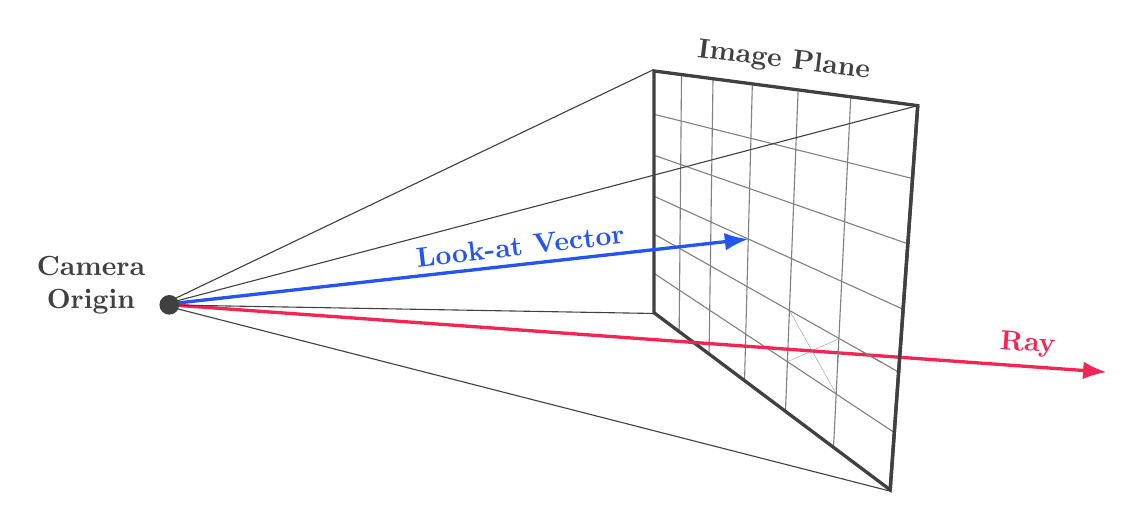
\begin{tikzpicture}[scale=1.0, every node/.style={scale=1.0}]
        % Plane inner lines
        \draw[-, color=gray, thin] (6.25, 2.42) -- (9.55, 1.6);
        \draw[-, color=gray, thin] (6.25, 1.9) -- (9.46, 0.78);
        \draw[-, color=gray, thin] (6.25, 1.38) -- (9.4, -0.05);
        \draw[-, color=gray, thin] (6.25, 0.9) -- (9.35, -0.85);
        \draw[-, color=gray, thin] (6.25, 0.4) -- (9.3, -1.62);

        \draw[-, color=gray, thin] (6.6, 2.92) -- (6.57, -0.35);
        \draw[-, color=gray, thin] (7, 2.87) -- (6.95, -0.63);
        \draw[-, color=gray, thin] (7.5, 2.82) -- (7.4, -0.98);
        \draw[-, color=gray, thin] (8.08, 2.7) -- (7.92, -1.35);
        \draw[-, color=gray, thin] (8.75, 2.65) -- (8.53, -1.82);

        % Pixel diagonals 
        \draw[-, color=gray, ultra thin] (7.95, -0.72) -- (8.6, -0.43);

        % Plane outer lines
        \draw[-, color=darkgray, very thick] (6.25, 2.97) -- (9.6, 2.53)
        -- (9.25, -2.35) -- (6.25, -0.1) -- (6.25, 2.97) -- (9.6, 2.53);
        \node[color=darkgray, rotate=-7] (x) at (7.9, 3.1) {\textbf{Image Plane}};

        % Looking direction vector
        \draw[-{Latex[length=3mm]}, color=axis_blue, very thick] (0.037, 0.005) -- (7.45, 0.835);
        \node[color=axis_blue, rotate=6.6] (x) at (4.55, 0.75) {\textbf{Look-at Vector}};

        % Ray 
        \draw[-{Latex[length=3mm]}, color=axis_red, very thick] (0.037, 0.005) -- (12, -0.855);
        \node[color=axis_red, rotate=-4] (x) at (11, -0.5) {\textbf{Ray}};

        % Camera to plane lines
        \draw[-, color=darkgray, thin] (0, 0) -- (6.235, 2.982);
        \draw[-, color=darkgray, thin] (0, 0) -- (9.6, 2.53);
        \draw[-, color=darkgray, thin] (0, 0) -- (9.25, -2.366);
        \draw[-, color=darkgray, thin] (0, 0) -- (6.25, -0.11);

        % Overlays over the ray
        \draw[{Round Cap[]}-{Round Cap[]}, color=gray, thin] (8.883, -0.5862) -- (9.15, -0.737);
        \draw[{Round Cap[]}-{Round Cap[]}, color=gray, thin] (8.593, -0.54) -- (8.583, -0.737);
        \draw[-, color=darkgray, very thick] (9.6, 2.53) -- (9.25, -2.35);

        % Pixel diagonals 
        \draw[-, color=gray, ultra thin] (7.973, -0.075) -- (8.57, -1.143);

        % Camera origin
        \node[fill=darkgray, circle, inner sep=0pt, minimum size=2.5mm] (c) at (0.95mm, 0) {};
        \node[color=darkgray, align=center] (x) at (-0.9, 0.25) {\textbf{Camera} \\ \textbf{Origin}};

    \end{tikzpicture}

    % Bottom margin
    \vspace{1cm}

    \caption[Visualization of a camera's image plane]{
        \centering
        Visualization of a camera's image plane, with a ray extending through a single pixel. Squares in the plane symbolize individual pixels in the rendered image. 
    }
    \label{fig:Implementation/RayGeneration/iamge_plane}
\end{figure}
\vfill

In a class defining a simplified camera model, we can introduce the functionality of calculating ray directions with a dedicated \verb|Camera::GetRayDirections| method. 
This method, can be declared to accept (as a parameter) an array of vectors, which will be populated with subsequent ray directions for every pixel in the output image.
Consequently, additional \verb|width| and \verb|height| parameters should be defined, which will specify the dimensions of the image, as well as the array's size.
\cref{lst:Implementation/RayGeneration/camera} demonstrates an example \verb|Camera| class declaration, constructed basing on the described methodology.

\vfill
\begin{figure}
    \lstinputlisting[
        xleftmargin=2em, 
        caption={[Basic \texttt{Camera} class declaration]
            Basic \texttt{Camera} class declaration.},
        label={lst:Implementation/RayGeneration/camera}
    ]{include/listings/ListingCamera1.cpp}
\end{figure}
\clearpage

\subsection{Transformation Matrices}

In order to convert individual screen-space pixel coordinates to ray directions, we'll first need to transform them into the world-space.
A common solution to this problem in computer graphics is to use an \textit{inverse view-projection matrix}, used for transforming vertices in screen-space into the world-space.
Usually denoted as $ (\bm{VP})^{-1} $, it is defined as the mathematical inverse of combined view and projection matrices.
Let's consider a point $ \bm{C}_{\textnormal{\small screen}} $ as a certain coordinate in screen-space.
The transformation to obtain a corresponding point $ \bm{C}_{\textnormal{\small world}} $ in world-space can be expressed as:
%
\begin{equation}
    \bm{C}_{\textnormal{\small world}} = (\bm{VP})^{-1} \cdot \bm{C}_{\textnormal{\small screen}} = (\bm{P}^{-1} \bm{V}^{-1}) \cdot \bm{C}_{\textnormal{\small screen}}
\end{equation}

To calculate an inverse view-projection matrix, we first need to construct a view matrix, which defines the intermediate step of transforming world-space coordinates into the camera's local space.
View matrices are often used in rasterization engines, to represent scene geometry relatively to a camera's position and orientation.
It can therefore be built using four vectors: the camera's world-space $ position $, along with three unit vectors, $ right $, $ up $, and $ forward $, which represent the camera's orientation:
%
\begin{equation}
    \bm{V} =
    \begin{bmatrix}
        right_x & up_x & forward_x & position_x\\
        right_y & up_y & forward_y & position_y\\
        right_z & up_z & forward_z & position_z\\
        0       & 0    & 0         & 1
    \end{bmatrix}
    \label{eq:Implementation/RayGeneration/view_matrix}
\end{equation}
%
However, since our goal is to only calculate ray directions, we can assume the camera is positioned at the world's origin, and just focus on its orientation.
Knowing the $ forward $ (looking) direction, the $ right $ and $ up $ vectors can be calculated in relation to the world's up (positive y-axis) direction, using vector cross products:  
%
{
    \newcommand*{\worldup}{\begin{bmatrix} 0 & 1 & 0 \end{bmatrix}\tran}
    \begin{align}
        right &= - \frac{forward\times\worldup}{\norm{forward\times\worldup}}\\[0.5em]
        up    &= - right \times forward
    \end{align}
    
}

Above equations aid us in implementing a view matrix creation function, seen in \cref{lst:Implementation/RayGeneration/view_matrix}.
Notice how the $ up $ vector gets negated in the function, as opposed to the general definition in \cref{eq:Implementation/RayGeneration/view_matrix}.
This is because ray directions are flipped on the y-axis in relation to screen-space pixel coordinates.
In YART, the $ y $ component of pixel coordinates increase when moving from top to bottom, whereas the ray pitch rotation should instead decrease.
The matrix returned from this function can later be inverted, ultimately resulting in the desired view matrix inverse.

\clearpage
\begin{figure}[!ht]
    \lstinputlisting[
        aboveskip=1\bigskipamount,
        xleftmargin=2em, 
        caption={[Implementation of a view matrix creation function]
            Implementation of a view matrix creation function.},
        label={lst:Implementation/RayGeneration/view_matrix}
    ]{include/listings/ListingViewMatrix.cpp}
\end{figure}

The next step in calculating a view-projection inverse is the definition of an \textit{inverse projection matrix}.
It is used in 3D computer graphics for transforming screen-space coordinates into camera-space.
Inverse projection matrices can be defined in numerous ways depending on the system's requirements.
In YART, this matrix is responsible for normalizing screen coordinates and centering them on the \textit{near clipping plane}. 
The near clipping plane is a mathematical plane placed in front of the camera, which determines how much of the scene should be \textit{clipped}, or hidden for rendering.
Given the output image dimensions $ (w, h) $ , and the near plane's distance $ d $, the inverse projection matrix $ \bm{P}^{-1} $ can be defined as follows:
%
\begin{equation}
    \newcommand*{\s}{\hspace{0.7em}}
    \bm{P}^{-1} =
    \begin{bmatrix}
        2u / w & 0      & \s 0 \s & \s 0 \s \\
        0      & 2v / h & 0       & 0       \\
        -u     & -v     & d       & 0       \\
        0      & 0      & 0       & 1
    \end{bmatrix},
    \label{eq:Implementation/RayGeneration/inverse_projection_matrix}
\end{equation}
%
where $ (u, v) $ are half the dimensions of the clipping plane, for a specified horizontal camera field of view in radians $ fov $:
%
\begin{align}
    u &= d \cdot \tan(fov / 2),\label{eq:Implementation/RayGeneration/u}\\[0.5em]
    v &= u \cdot h/w \label{eq:Implementation/RayGeneration/v}
\end{align}

\cref{lst:Implementation/RayGeneration/ip_matrix} demonstrates an example inverse projection matrix creation function based on Equations (\ref{eq:Implementation/RayGeneration/inverse_projection_matrix}\textendash\ref{eq:Implementation/RayGeneration/v}).

\begin{figure}[!ht]
    \lstinputlisting[
        xleftmargin=2em, 
        caption={[Implementation of an inverse projection matrix creation function]
            Implementation of an inverse projection matrix creation function.},
        label={lst:Implementation/RayGeneration/ip_matrix}
    ]{include/listings/ListingInverseProjectionMatrix.cpp}
\end{figure}


\subsection{Calculating Ray Directions}

Functions outlined in Listings \ref{lst:Implementation/RayGeneration/camera}--\ref{lst:Implementation/RayGeneration/ip_matrix} can be used in combination to develop a simple ray generation procedure.
The computed view matrix can be inverted and combined with the inverse projection matrix to construct an inverse view-projection matrix.
This matrix will ultimately be used for transforming screen-space pixel coordinates into ray directions.
\cref{lst:Implementation/RayGeneration/ray_generation} proposes an example implementation of such functionality, in the form of the \verb|Camera| class's \verb|GetRayDirections| method.
Subsequent $ (x, y) $ pixel coordinates are offset by half an unit to obtain their centers, and applied to the inverse view-projection matrix. 
Finally, the vectors get truncated into three dimensions and normalized, resulting in the desired ray directions.

\vfill
\begin{figure}[!ht]
    \lstinputlisting[
        xleftmargin=2em, 
        caption={[\texttt{Camera::GetRayDirections} method implementation]
            \texttt{Camera::GetRayDirections} method implementation.},
        label={lst:Implementation/RayGeneration/ray_generation}
    ]{include/listings/ListingRayGeneration1.cpp}
\end{figure}
\vfill

\subsection{Ray Direction Caching}

A number of optimization techniques can be applied to the ray generation procedure, which can greatly impact its performance. 
One notable example involves the utilization of a caching mechanism, a strategy employed in the YART engine.
It is built on the key observation, that once calculated ray directions may be cached under certain conditions and reused between subsequent frames.
As seen in \cref{lst:Implementation/RayGeneration/ray_generation}, our implementation of ray generation depends on just a couple of variables: the camera's looking direction, FOV, and the output image's size.
Consequently, change in the camera's position, as well as changes not directly related to the camera, should not require the ray directions to be recalculated. 
They can therefore be stored in memory and reused until specific camera properties are modified, or the screen is resized.
The current \verb|Camera| class implementation can be slightly altered to reflect this methodology, as seen in \cref{lst:Implementation/RayGeneration/camera_caching}.

\vfill
\begin{figure}[!ht]
    \lstinputlisting[
        xleftmargin=2em, 
        caption={[Modified \texttt{Camera} class declaration for ray direction caching]
            Modified \texttt{Camera} class declaration for ray direction caching.},
        label={lst:Implementation/RayGeneration/camera_caching}
    ]{include/listings/ListingCamera2.cpp}
\end{figure}
\vfill

The resizable cache, along with its current dimensions, can be stored as private members within the \verb|Camera| class.
Additionally, a \verb|Camera::RecalculateCache| method can be introduced.
It will be used under certain conditions for recalculating the ray directions cache. 
This method has intentionally been declared to mirror the definition of \verb|Camera::GetRayDirections|, presented in \cref{lst:Implementation/RayGeneration/ray_generation}, as its implementation can effectively be reused for this task.
Conversely, the method for retrieving ray directions should be redefined to reflect this change (see \cref{lst:Implementation/RayGeneration/ray_generation_cache}).

\vfill
\begin{figure}[!ht]
    \lstinputlisting[
        xleftmargin=2em, 
        caption={[Modified \texttt{Camera::GetRayDirections} method implementation]
            Modified \texttt{Camera::GetRayDirections} method implementation.},
        label={lst:Implementation/RayGeneration/ray_generation_cache}
    ]{include/listings/ListingRayGeneration2.cpp}
\end{figure}
\vfill

In the modified version of the \verb|Camera::GetRayDirections| method, ray directions are returned from the cache, which only gets recalculated when a change in screen resolution is detected.
This methodology can later be extended upon, to recalculate the cache when the camera's rotation or field of view changes, possibly with the use of property setters and additional state.  

\section{Scene Representation}

mesh definition, normals calculation, uv coordinates, sphere mesh generation(?), light objects

\dots

\section{Intersection Testing, Materials, and Shading}

Möller-Trumbore algorithm for tri-ray intersection, solid color materials, shading using blinn-phong reflection model

\dots

\section{Sky Color Sampling}

solid color skies, linear gradients, and cubemap skyboxes

\dots

\section{Shadows}

hard shadows implementation

\dots

\section{Bounding Volume Hierarchies}

optimization strategies using BVH trees, AABB tree implementation

\dots

        %--------------------------------------------------------------------------------------------
%   YART thesis "Conclusion" chapter definition.
%--------------------------------------------------------------------------------------------

\chapter{Conclusion} \label{ch:Conclusion}

\dots

\section{Tests and Case Studies}

\dots

\section{Limitations and Future Work}

\dots

\section{Further Reading}

\dots

    % \end{onehalfspace}

    % List of figures
    \clearpage\phantomsection
    \addcontentsline{toc}{chapter}{\MakeUppercase\listfigurename}
    \listoffigures

    % List of listings
    \clearpage\phantomsection
    \addcontentsline{toc}{chapter}{\MakeUppercase\lstlistlistingname}
    \lstlistoflistings

    % BibTeX references
    \renewcommand\bibname{References}
    \printbibliography
    \addcontentsline{toc}{chapter}{\MakeUppercase\bibname}

\end{document}
